\chapter{Spektroskopi untuk Menentukan Struktur}\label{ch:b1:structure-spectroscopy}

Seorang peracik parfum menyerahkan kepada laboratorium sebuah cairan tak
berwarna yang berbau nanas dan bertanya zat apakah itu. Lima puluh tahun
yang lalu, jawabannya memerlukan berminggu-minggu reaksi penguraian.
Sekarang cukup sepuluh menit: analisis unsur memberikan rumusnya,
spektrum inframerah menunjukkan gugus fungsinya, dan spektrum resonansi
magnetik inti proton memperlihatkan bagaimana atom-atomnya terhubung.
Bab ini menjelaskan cara membaca setiap spektrum --- apa yang dilakukan
cahaya dari setiap daerah terhadap sebuah molekul, dan ciri spektrum
mana yang membawa potongan struktur mana --- dan ditutup dengan molekul
nanas itu.

\begin{recall}
Jilid sekolah (kelas 11 dan 12) mengukur \omterm{def:b1:structure-spectroscopy:absorbance}{absorbans} dengan
spektrofotometer dan memakai hukum Beer--Lambert untuk menentukan
konsentrasi, mengenali gugus fungsi dari tabel pita inframerah, dan
membaca spektrum NMR proton yang sederhana (banyaknya sinyal, \omterm{def:b1:structure-spectroscopy:integration}{integrasi},
aturan $n + 1$). Ikatan tunggal, rangkap dua, dan rangkap tiga serta
ikatan $\pi$ adalah yang pada \cref{ch:b1:lewis-resonance-vsepr}.
\end{recall}

\section{Spektroskopi UV--tampak: konjugasi dan warna}

\begin{definition}[Absorbans dan hukum Beer--Lambert]\label{def:b1:structure-spectroscopy:absorbance}
Untuk cahaya berintensitas $I_0$ yang memasuki sebuah larutan dan $I$
yang keluar darinya, \emph{absorbans}\index{absorbans} adalah
$A = \log(I_0/I)$. Untuk larutan encer satu spesies penyerap,
$A = \varepsilon\,\ell\,c$ (hukum Beer--Lambert), dengan $\ell$ panjang
lintasan, $c$ konsentrasi, dan $\varepsilon$ \emph{koefisien absorpsi
molar}\index{koefisien absorpsi molar}, sifat spesies itu pada panjang
gelombang tersebut.
\end{definition}

Sebuah molekul menyerap cahaya ultraungu atau cahaya tampak jika energi
foton sama dengan celah antara tingkat elektron terisi tertinggi dan
tingkat kosong terendah ikatan-ikatannya. Untuk ikatan $\sigma$ celahnya
besar dan serapannya jauh di daerah ultraungu; ikatan $\pi$ menyerap
lebih dekat ke cahaya tampak, dan rantai ikatan rangkap dua dan tunggal
yang berselang-seling menyerap pada panjang gelombang yang makin panjang
seiring makin panjangnya rantai.

\begin{definition}[Sistem terkonjugasi, kromofor, maksimum serapan]\label{def:b1:structure-spectroscopy:conjugation}
\emph{Sistem terkonjugasi}\index{sistem terkonjugasi} adalah rantai atom
yang masing-masing membawa orbital $p$ dalam sebuah sistem $\pi$, seperti
pada ikatan rangkap dua dan tunggal yang berselang-seling
(buta-1,3-diena, benzena). Gugus atom yang bertanggung jawab atas
sebuah serapan adalah \emph{kromofor}\index{kromofor} serapan itu; panjang
gelombang tempat \omterm{def:b1:structure-spectroscopy:absorbance}{absorbansnya} paling besar adalah \emph{maksimum
serapan}\index{maksimum serapan}, $\lambda_{\max}$.
\end{definition}

Tingkat-tingkat sebuah \omterm{def:b1:structure-spectroscopy:conjugation}{sistem terkonjugasi} tersebar di seluruh rantai dan
makin berdekatan seiring bertambah panjangnya rantai, seperti
tingkat-tingkat sebuah partikel dalam kotak yang lebih panjang:
$\lambda_{\max}$ bertambah dengan konjugasi. Etena dan butadiena hanya
menyerap di daerah ultraungu; sebelas ikatan rangkap dua terkonjugasi
$\beta$-karoten membawa serapannya ke bagian biru cahaya tampak. Sebuah
zat tampak berwarna komplementer dari cahaya yang diserapnya: karena
menyerap biru dan ungu, karoten tampak jingga.

\begin{omfigure}
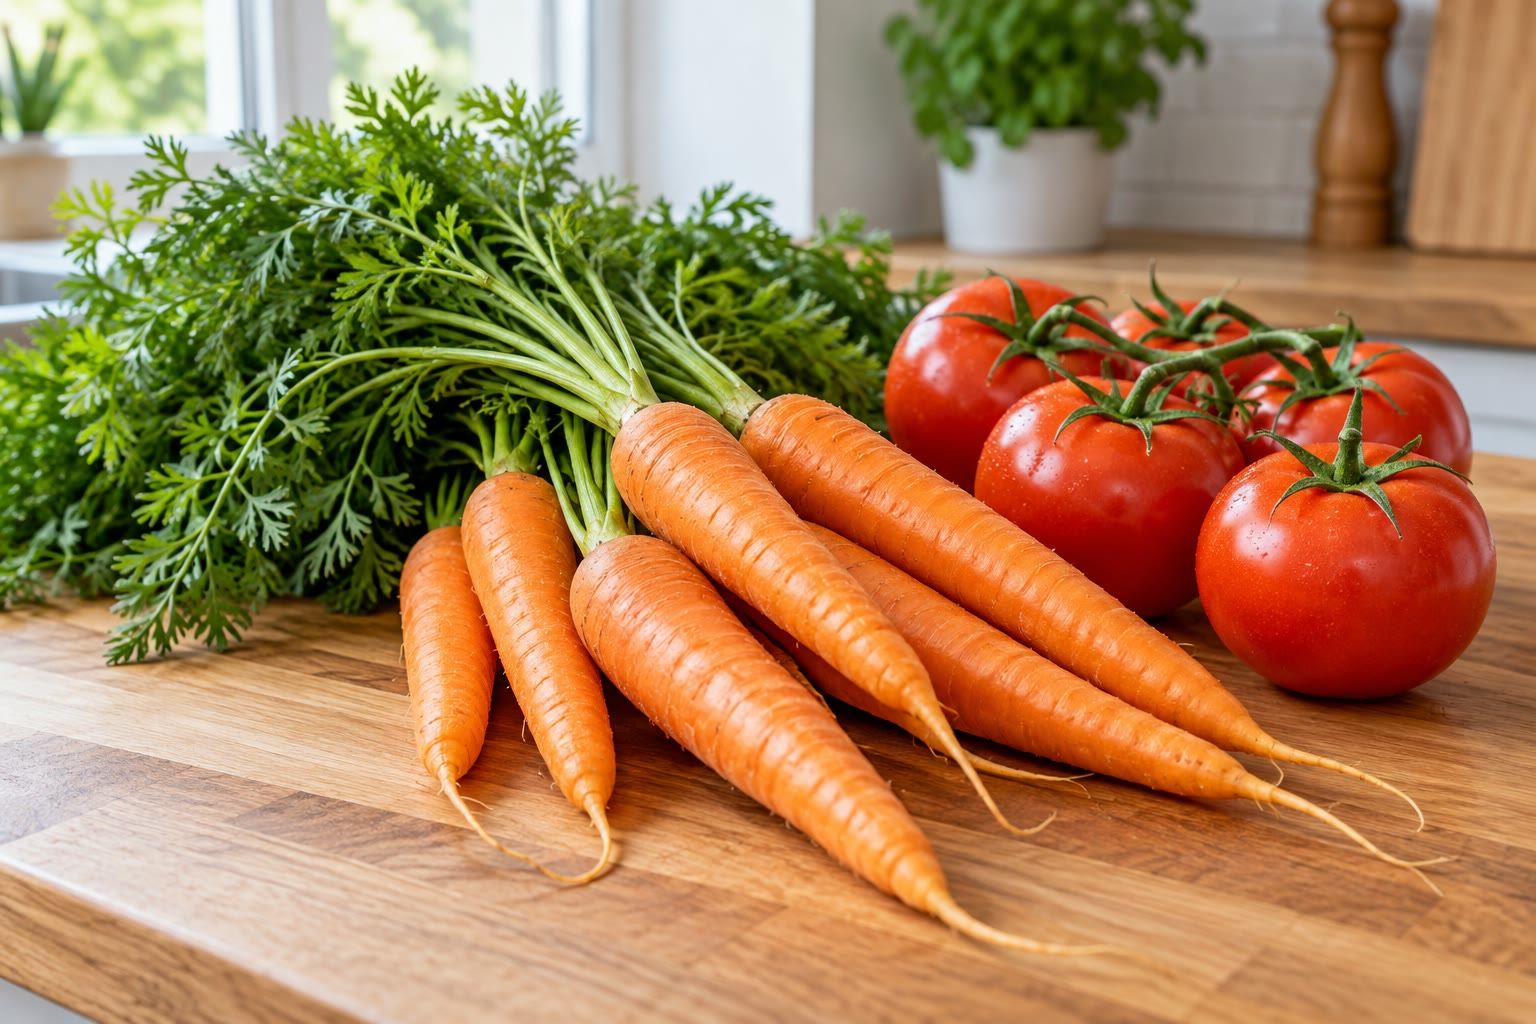
\includegraphics[width=0.55\linewidth]{images/book2/ai/b1-17-carrots-tomatoes.jpg}

{\small Wortel dan tomat mendapatkan warnanya dari molekul-molekul
terkonjugasi yang panjang, karoten dan likopena, yang menyerap cahaya
biru dan hijau serta meneruskan jingga dan merah.}
\end{omfigure}

\begin{omfigure}
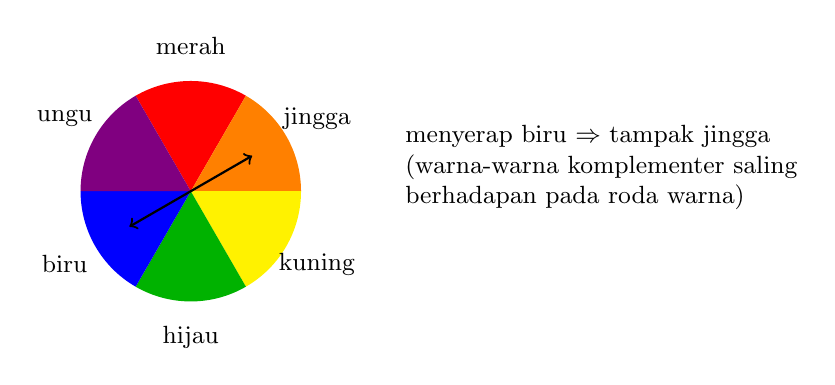
\begin{tikzpicture}[font=\small]
  \foreach \a/\c/\n in {90/red/merah, 30/orange/jingga, -30/yellow/kuning, -90/green!70!black/hijau, -150/blue/biru, 150/violet/ungu} {
    \fill[\c] (0,0) -- (\a-30:1.4) arc[start angle=\a-30, end angle=\a+30, radius=1.4] -- cycle;
    \node at (\a:1.85) {\n};
  }
  \draw[<->, thick] (-150:0.9) -- (30:0.9);
  \node[align=left, anchor=west] at (2.6,0.3) {menyerap biru $\Rightarrow$ tampak jingga\\(warna-warna komplementer saling\\berhadapan pada roda warna)};
\end{tikzpicture}

{\small Sebuah roda warna. Warna yang terlihat adalah komplemen warna yang
diserap: larutan yang menyerap di daerah biru tampak jingga.}
\end{omfigure}

\section{Spektroskopi inframerah lebih mendalam}

\begin{definition}[Bilangan gelombang, transmitans, daerah sidik jari]\label{def:b1:structure-spectroscopy:wavenumber}
Spektrum inframerah digambar terhadap \emph{bilangan
gelombang}\index{bilangan gelombang} $\tilde\nu = 1/\lambda$, dalam
\unit{cm^{-1}}, yang sebanding dengan energi foton. Ordinatnya adalah
\emph{transmitans}\index{transmitans} $T = I/I_0$, dalam persen, sehingga
pita-pitanya mengarah ke bawah. Di bawah sekitar \qty{1500}{cm^{-1}}
banyak pita yang saling tumpang tindih, yang khas bagi seluruh molekul
dan bukan bagi satu ikatan, membentuk \emph{daerah sidik
jari}\index{daerah sidik jari}.
\end{definition}

Sebuah ikatan menyerap cahaya inframerah pada frekuensi getarannya.
Seperti dua massa yang dihubungkan oleh sebuah pegas, makin kaku ikatan
itu dan makin ringan atom-atomnya, makin tinggi \omterm{def:b1:structure-spectroscopy:wavenumber}{bilangan gelombangnya}:
ikatan dengan hidrogen (O--H, C--H) di atas \qty{2800}{cm^{-1}}, ikatan
rangkap tiga di dekat 2200, ikatan rangkap dua di dekat 1700--1600,
ikatan tunggal antara atom-atom yang lebih berat di bawah 1300. Tabel ini
memberikan posisi terukur untuk molekul-molekul dalam bab ini, dalam \omterm{def:b1:extent-q-and-k:system}{fase}
gas, tempat molekul-molekulnya terisolasi.

\begin{omfigure}
\begin{tabular}{llr}
\hline
molekul & ikatan & $\tilde\nu$ (\unit{cm^{-1}}) \\
\hline
etanol & O--H & 3666 \\
etanol & C--H & 2978 \\
etanol & C--O & 1060 \\
propanon & C=O & 1738 \\
asam etanoat & O--H & 3582 \\
asam etanoat & C=O & 1788 \\
etil etanoat & C=O & 1764 \\
etil etanoat & C--O & 1238 \\
\hline
\end{tabular}

\smallskip
{\small Maksimum pita dalam spektrum inframerah \omterm{def:b1:extent-q-and-k:system}{fase} gas. Dalam zat cair,
\omterm{def:b1:intermolecular-forces-solvents:hbond}{ikatan hidrogen} melebarkan pita O--H dan menggesernya ke \omterm{def:b1:structure-spectroscopy:wavenumber}{bilangan
gelombang} yang lebih rendah, dan pita C=O asam bergeser turun ketika
asam itu berpasangan.}
% ledger: ir:ethanol-OH, ir:ethanol-CH, ir:ethanol-CO, ir:propanone-CO, ir:ethanoic-OH, ir:ethanoic-CO, ir:ethylethanoate-CO, ir:ethylethanoate-COC
\end{omfigure}

\begin{omfigure}
\begin{tikzpicture}
\begin{axis}[name=i1, width=0.86\linewidth, height=3.2cm, xmin=500, xmax=4000, x dir=reverse, ymin=0, ymax=105, ytick={0,50,100}, ylabel={$T$ (\%)}, tick label style={font=\scriptsize}, label style={font=\small}, xticklabels={}]
\addplot[omDef, thick] table[x=nu, y=T] {figdata/out/bachelor-1-spectra-ir-ethanol.dat};
\node[font=\scriptsize, anchor=west] at (axis cs:2600,25) {etanol};
\end{axis}
\begin{axis}[name=i2, at={(i1.south)}, anchor=north, yshift=-0.25cm, width=0.86\linewidth, height=3.2cm, xmin=500, xmax=4000, x dir=reverse, ymin=0, ymax=105, ytick={0,50,100}, ylabel={$T$ (\%)}, tick label style={font=\scriptsize}, label style={font=\small}, xticklabels={}]
\addplot[omProp, thick] table[x=nu, y=T] {figdata/out/bachelor-1-spectra-ir-propanone.dat};
\node[font=\scriptsize, anchor=west] at (axis cs:2600,25) {propanon};
\end{axis}
\begin{axis}[at={(i2.south)}, anchor=north, yshift=-0.25cm, width=0.86\linewidth, height=3.2cm, xmin=500, xmax=4000, x dir=reverse, ymin=0, ymax=105, ytick={0,50,100}, ylabel={$T$ (\%)}, tick label style={font=\scriptsize}, label style={font=\small}, xlabel={bilangan gelombang (\unit{cm^{-1}})}]
\addplot[omMeth, thick] table[x=nu, y=T] {figdata/out/bachelor-1-spectra-ir-ethanoic.dat};
\node[font=\scriptsize, anchor=west] at (axis cs:2600,25) {asam etanoat};
\end{axis}
\end{tikzpicture}

{\small Spektrum inframerah etanol, propanon, dan asam etanoat, yang
disimulasikan dari posisi pita terukur dalam tabel (tinggi dan lebar
pita skematis). Pita C=O di dekat \qty{1750}{cm^{-1}} dan pita O--H di
atas \qty{3500}{cm^{-1}} membedakan ketiga gugus fungsi itu dalam
sekilas pandang.}
\end{omfigure}

\section{NMR proton: pergeseran kimia dan integrasi}

Dalam medan magnet yang kuat, sebuah proton mempunyai dua \omterm{def:b1:quantum-numbers:energy-level}{tingkat energi};
gelombang radio dengan frekuensi yang tepat membuatnya berbalik dari yang
satu ke yang lain. Frekuensi itu sebanding dengan medan magnet yang
benar-benar dirasakan proton, yang sedikit dikurangi oleh
elektron-elektron di sekitarnya. Karena itu proton-proton dalam
lingkungan kimia yang berbeda beresonansi pada frekuensi yang sedikit
berbeda.

\begin{definition}[Pergeseran kimia, efek perisai, proton ekuivalen]\label{def:b1:structure-spectroscopy:chemical-shift}
\emph{Pergeseran kimia}\index{pergeseran kimia} sebuah proton adalah
$\delta = (\nu - \nu_{\text{acuan}})/\nu_0 \times 10^6$, dalam \unit{ppm},
dengan $\nu$ frekuensi resonansinya, $\nu_{\text{acuan}}$ frekuensi
resonansi proton-proton tetrametilsilana, dan $\nu_0$ frekuensi kerja
spektrometer. Pengurangan medan pada sebuah inti oleh elektron-elektronnya
adalah \emph{efek perisai}\index{efek perisai} inti itu: tetangga-tetangga
penarik elektron (O, halogen, C=O) mengurangi perisai sebuah proton dan
menaikkan $\delta$-nya. \emph{Proton ekuivalen}\index{proton ekuivalen}
adalah proton-proton yang dipertukarkan oleh suatu simetri molekul atau
oleh rotasi yang cepat; proton-proton itu mempunyai pergeseran yang
sama.
\end{definition}

\begin{proposition}[Pergeseran tidak bergantung pada spektrometer]\label{prop:b1:structure-spectroscopy:shift-field-independent}
\omterm{def:b1:structure-spectroscopy:chemical-shift}{Pergeseran kimia} sebuah proton sama pada spektrometer-spektrometer
dengan medan yang berbeda.
\end{proposition}

\begin{proof}
Baik $\nu$ maupun $\nu_{\text{acuan}}$ sebanding dengan medan yang
diterapkan $B_0$ (masing-masing dikalikan dengan faktor perisainya
sendiri), demikian pula $\nu_0$. Karena itu rasio
$(\nu - \nu_{\text{acuan}})/\nu_0$ tidak bergantung pada $B_0$.
Sebaliknya, selisih dalam hertz bertambah dengan medan.
\end{proof}

\begin{definition}[Integrasi]\label{def:b1:structure-spectroscopy:integration}
\emph{Integrasi}\index{integrasi} sebuah sinyal adalah luasnya, yang
dibaca pada spektrum sebagai tinggi sebuah kurva bertangga; luas-luas
itu sebanding dengan banyaknya proton yang memberikan sinyal-sinyal
tersebut.
\end{definition}

\section{Kopling spin--spin}

\begin{definition}[Kopling spin--spin, tetapan kopling, multiplet]\label{def:b1:structure-spectroscopy:coupling}
Melalui ikatan-ikatan, keadaan magnetik sebuah proton sedikit mengubah
medan yang dirasakan proton-proton pada karbon-karbon tetangganya:
\emph{kopling spin--spin}\index{kopling spin--spin} ini memecah setiap
sinyal menjadi sebuah \emph{multiplet}\index{multiplet} yang
garis-garisnya terpisah sejauh
\emph{tetapan kopling}\index{tetapan kopling} $J$, dalam hertz. Dua proton yang saling berkopling
memperlihatkan $J$ yang sama; proton-proton ekuivalen tidak saling
memecah sinyalnya.
\end{definition}

\begin{proposition}[Aturan \texorpdfstring{$n + 1$}{n + 1}]\label{prop:b1:structure-spectroscopy:n-plus-one}
Sebuah proton (atau sekumpulan \omterm{def:b1:structure-spectroscopy:chemical-shift}{proton ekuivalen}) yang berkopling dengan
$J$ yang sama pada $n$ tetangga ekuivalen memberikan $n + 1$ garis,
terpisah sejauh $J$, dengan intensitas relatif sama dengan koefisien
binomial $\binom{n}{k}$, $k = 0$ sampai $n$ (\emph{aturan
$n + 1$}\index{aturan $n + 1$}).
\end{proposition}

\begin{proof}
Setiap tetangga berada dalam salah satu dari dua keadaan spin, yang
menggeser garis yang teramati sebesar $+J/2$ atau $-J/2$. Dengan $n$
tetangga pergeserannya $(k - n/2)J$, dengan $k$ banyaknya tetangga dalam
keadaan pertama: $n + 1$ nilai, berjarak sama sebesar $J$. Karena kedua
keadaan itu hampir sama banyak penghuninya, semua $2^n$ kombinasi sama
peluangnya, dan $k$ di antaranya berada dalam keadaan pertama dalam
$\binom{n}{k}$ cara.
\end{proof}

\begin{omfigure}
\begin{tikzpicture}[font=\small, x=0.85cm, y=0.5cm]
  % quartet: three neighbours, each split +-J/2 (J = 1.5 units)
  \draw[thick] (0,4) -- (0,3.4);
  \foreach \x in {-0.75,0.75} \draw (0,3.4) -- (\x,2.4);
  \foreach \a/\b in {-0.75/-1.5, -0.75/0, 0.75/0, 0.75/1.5} \draw (\a,2.4) -- (\b,1.4);
  \foreach \a/\b in {-1.5/-2.25, -1.5/-0.75, 0/-0.75, 0/0.75, 1.5/0.75, 1.5/2.25} \draw (\a,1.4) -- (\b,0.4);
  \foreach \x/\h in {-2.25/1, -0.75/3, 0.75/3, 2.25/1} {\draw[omDef, very thick] (\x,-2.6) -- (\x,{-2.6+0.7*\h}); \draw[dotted] (\x,0.4) -- (\x,{-2.6+0.7*\h});}
  \draw (-2.8,-2.6) -- (2.8,-2.6);
  \node at (0,-3.4) {kuartet 1\,:\,3\,:\,3\,:\,1 (\ce{-CH2-} di sebelah \ce{-CH3})};
  % triplet: two neighbours
  \begin{scope}[xshift=7.5cm]
  \draw[thick] (0,4) -- (0,3.4);
  \foreach \x in {-0.75,0.75} \draw (0,3.4) -- (\x,2.4);
  \foreach \a/\b in {-0.75/-1.5, -0.75/0, 0.75/0, 0.75/1.5} \draw (\a,2.4) -- (\b,1.4);
  \foreach \x/\h in {-1.5/1, 0/2, 1.5/1} {\draw[omProp, very thick] (\x,-2.6) -- (\x,{-2.6+0.7*\h}); \draw[dotted] (\x,1.4) -- (\x,{-2.6+0.7*\h});}
  \draw (-2.1,-2.6) -- (2.1,-2.6);
  \draw[<->] (-1.5,-0.6) -- (0,-0.6) node[midway, above, font=\scriptsize] {$J$};
  \node at (0,-3.4) {triplet 1\,:\,2\,:\,1 (\ce{-CH3} di sebelah \ce{-CH2-})};
  \end{scope}
\end{tikzpicture}

{\small Pohon pemecahan. Setiap tetangga memecah setiap garis menjadi dua,
yang berjarak $J$; garis-garis yang berimpit saling menjumlah,
menghasilkan intensitas binomial.}
\end{omfigure}

\begin{omfigure}
\begin{tikzpicture}
\begin{axis}[name=ea,
  width=0.86\linewidth, height=4.2cm, xmin=0.8, xmax=4.5, x dir=reverse, ymin=0, ymax=1.15,
  axis x line=bottom, axis y line=none, xlabel={$\delta$ (ppm)},
  tick label style={font=\scriptsize}, label style={font=\small}]
\addplot[omDef, thin] table[x=ppm, y=I] {figdata/out/bachelor-1-spectra-nmr-ethylethanoate.dat};
\node[font=\scriptsize, anchor=south] at (axis cs:4.12,0.75) {q, 2H};
\node[font=\scriptsize, anchor=west] at (axis cs:2.0,0.95) {s, 3H};
\node[font=\scriptsize, anchor=west] at (axis cs:1.15,0.8) {t, 3H};
\node[font=\small, anchor=north] at (axis cs:3.0,1.1) {\ce{CH3COOCH2CH3}};
\end{axis}
\begin{axis}[at={(ea.south)}, anchor=north, yshift=-1.3cm,
  width=0.86\linewidth, height=4.2cm, xmin=0.8, xmax=4.5, x dir=reverse, ymin=0, ymax=1.15,
  axis x line=bottom, axis y line=none, xlabel={$\delta$ (ppm)},
  tick label style={font=\scriptsize}, label style={font=\small}]
\addplot[omProp, thin] table[x=ppm, y=I] {figdata/out/bachelor-1-spectra-nmr-ethanol.dat};
\node[font=\scriptsize, anchor=south] at (axis cs:3.69,0.75) {q, 2H};
\node[font=\scriptsize, anchor=west] at (axis cs:2.55,0.6) {s, 1H};
\node[font=\scriptsize, anchor=west] at (axis cs:1.1,0.8) {t, 3H};
\node[font=\small, anchor=north] at (axis cs:2.9,1.1) {\ce{CH3CH2OH}};
\end{axis}
\end{tikzpicture}

{\small Spektrum NMR proton etil etanoat (atas) dan etanol (bawah) dalam
\ce{CDCl3}, yang disimulasikan pada \qty{90}{MHz} dari pergeseran dan
\omterm{def:b1:structure-spectroscopy:coupling}{tetapan kopling} terukur ($J = \qty{7.2}{Hz}$ dan \qty{7.0}{Hz}). Kuartet
\ce{OCH2} kurang terperisai karena oksigen; pada etanol proton OH, yang
dipertukarkan dengan cepat antarmolekul, tidak berkopling dan
pergeserannya bergantung pada konsentrasi.}
% ledger: nmr:ethylethanoate-OCH2, nmr:ethylethanoate-COCH3, nmr:ethylethanoate-CH3, nmr:ethylethanoate-J, nmr:ethanol-CH2, nmr:ethanol-CH3, nmr:ethanol-OH, nmr:ethanol-J
\end{omfigure}

\begin{omfigure}
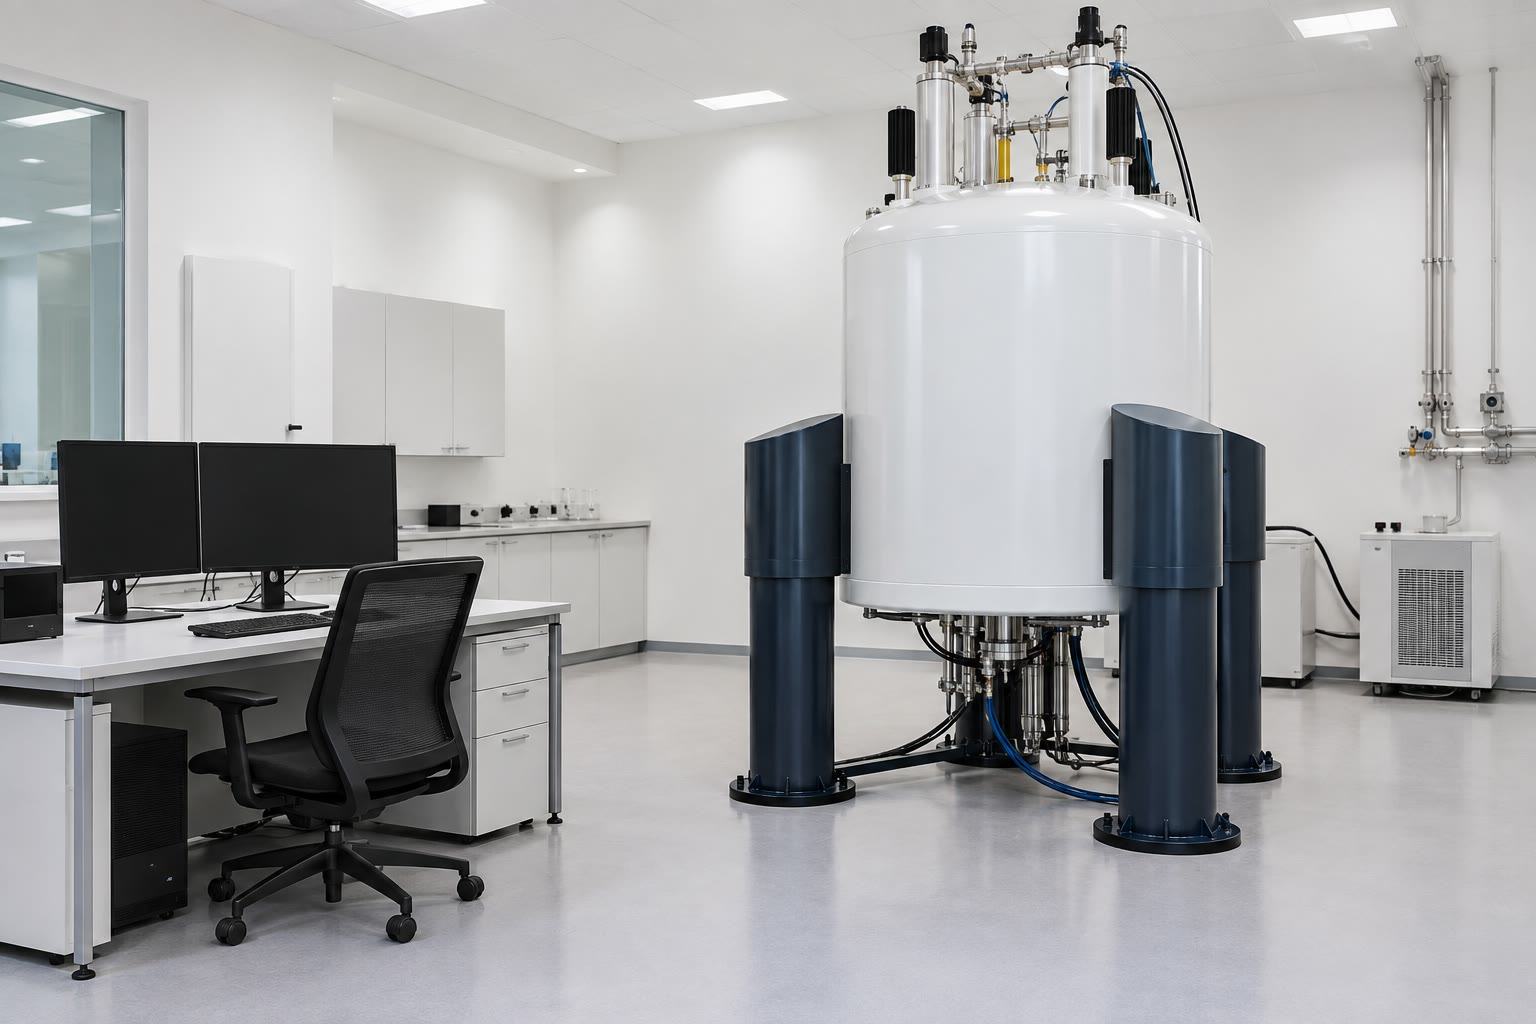
\includegraphics[width=0.5\linewidth]{images/book2/ai/b1-17-nmr.jpg}

{\small Sebuah spektrometer NMR: silinder tinggi itu menampung magnet
superkonduktor yang didinginkan dengan helium cair; tabung sampel
diturunkan ke pusatnya.}
\end{omfigure}

\section{Menentukan sebuah struktur}

\begin{definition}[Derajat ketidakjenuhan]\label{def:b1:structure-spectroscopy:unsaturation}
\emph{Derajat ketidakjenuhan}\index{derajat ketidakjenuhan} sebuah rumus
adalah banyaknya cincin ditambah banyaknya ikatan $\pi$ dalam molekul
itu.
\end{definition}

\begin{proposition}[Derajat ketidakjenuhan dari rumus]\label{prop:b1:structure-spectroscopy:unsaturation-formula}
Untuk molekul $\mathrm{C}_c\mathrm{H}_h\mathrm{N}_n\mathrm{O}_o\mathrm{X}_x$
(X sebuah halogen), \omterm{def:b1:structure-spectroscopy:unsaturation}{derajat ketidakjenuhannya} adalah
\[
  D = \frac{2c + 2 + n - h - x}{2} .
\]
\end{proposition}

\begin{proof}
Rantai terbuka $c$ karbon yang hanya berikatan tunggal membawa $2c + 2$
hidrogen. Setiap cincin atau ikatan $\pi$ mengurangi dua di antaranya.
Oksigen divalen yang disisipkan dalam rantai tidak mengubah apa pun;
nitrogen trivalen membawa satu hidrogen lagi; halogen menggantikan satu
hidrogen. Menghitung hidrogen yang hilang dan membaginya dengan dua
menghasilkan $D$.
\end{proof}

\begin{method}[Menentukan sebuah struktur]\label{met:b1:structure-spectroscopy:solve-structure}
\begin{enumerate}
  \item Dari rumusnya, hitunglah $D$.
  \item Dari spektrum IR, tentukan gugus-gugus fungsinya (C=O, O--H,
        N--H, C--O) dan ketiadaan gugus-gugus lain.
  \item Dari spektrum NMR: banyaknya sinyal (kumpulan \omterm{def:b1:structure-spectroscopy:chemical-shift}{proton ekuivalen}),
        \omterm{def:b1:structure-spectroscopy:integration}{integrasi} (proton per kumpulan), pergeseran (gugus tetangga),
        multiplisitas (banyaknya tetangga menurut aturan $n + 1$),
        \omterm{def:b1:structure-spectroscopy:coupling}{tetapan kopling} (sinyal mana yang bertetangga).
  \item Susunlah fragmen-fragmen, gabungkan, lalu periksalah setiap puncak
        terhadap struktur yang diusulkan; singkirkan isomer-isomer yang
        tidak sesuai.
\end{enumerate}
\end{method}

\section{Latihan}

\begin{exercise}[$\star$]\label{exo:b1:structure-spectroscopy:1}
Larutan sebuah zat warna \qty{2.0e-5}{mol/L} dalam kuvet \qty{1.00}{cm}
mempunyai \omterm{def:b1:structure-spectroscopy:absorbance}{absorbans} 0.64 pada \omterm{def:b1:structure-spectroscopy:conjugation}{maksimum serapannya}. Hitunglah
$\varepsilon$, dan \omterm{def:b1:structure-spectroscopy:absorbance}{absorbans} larutan yang tiga kali lebih pekat.
\end{exercise}

\begin{exercise}[$\star$]\label{exo:b1:structure-spectroscopy:2}
Hitunglah \omterm{def:b1:structure-spectroscopy:unsaturation}{derajat ketidakjenuhan} \ce{C6H6}, \ce{C4H8O2}, \ce{C3H7NO},
\ce{C2H3Cl}, dan \ce{C10H14O} (karvon). Usulkan satu struktur untuk
masing-masing.
\end{exercise}

\begin{exercise}[$\star$]\label{exo:b1:structure-spectroscopy:3}
Berapa banyak sinyal proton, dengan \omterm{def:b1:structure-spectroscopy:integration}{integrasi} berapa, yang diberikan oleh
propanon, asam etanoat, 2-metilpropana, dan 1,2-dikloroetana?
\end{exercise}

\begin{exercise}[$\star$]\label{exo:b1:structure-spectroscopy:4}
Sebuah sinyal terletak \qty{1460}{Hz} dari tetrametilsilana pada
spektrometer \qty{400}{MHz}. Berapa pergeserannya? Berapa jauhnya dalam
hertz pada \qty{90}{MHz}? Mengapa medan yang tinggi memisahkan
\omterm{def:b1:structure-spectroscopy:coupling}{multiplet-multiplet} dengan lebih baik?
\end{exercise}

\begin{exercise}[$\star\star$]\label{exo:b1:structure-spectroscopy:5}
Ramalkan multiplisitas setiap sinyal 1-bromopropana,
\ce{CH3CH2CH2Br}, dengan anggapan tetapan-tetapan koplingnya sama, serta
intensitas relatif garis-garis sinyal tengahnya.
\end{exercise}

\begin{exercise}[$\star\star$]\label{exo:b1:structure-spectroscopy:6}
Bagaimana spektrum IR etanol, propanon, dan asam etanoat berbeda antara
1700 dan \qty{3700}{cm^{-1}}? Senyawa manakah yang memberikan sekaligus
pita C=O dan pita O--H?
\end{exercise}

\begin{exercise}[$\star\star$]\label{exo:b1:structure-spectroscopy:7}
Dua isomer \ce{C4H8O2}: etil etanoat dan metil propanoat. Ramalkan
spektrum NMR-nya (pergeseran kira-kira, multiplisitas, \omterm{def:b1:structure-spectroscopy:integration}{integrasi}), lalu
nyatakan cara membedakan keduanya.
\end{exercise}

\begin{exercise}[$\star\star$]\label{exo:b1:structure-spectroscopy:8}
Dengan spektrum etil etanoat yang disimulasikan, bacalah jarak antara
dua garis kuartet dalam ppm lalu ubahlah menjadi hertz (spektrum itu
disimulasikan pada \qty{90}{MHz}). Bandingkan dengan tripletnya.
\end{exercise}

\begin{exercise}[$\star\star$]\label{exo:b1:structure-spectroscopy:9}
Sebuah senyawa \ce{C3H6O} memperlihatkan pita IR yang kuat pada
\qty{1738}{cm^{-1}} dan satu sinyal NMR. Tentukan senyawa itu. Isomer
manakah yang akan memperlihatkan pita di dekat \qty{2720}{cm^{-1}} dan
sinyal di dekat \qty{9.8}{ppm}?
\end{exercise}

\begin{exercise}[$\star\star\star$]\label{exo:b1:structure-spectroscopy:10}
Buktikan aturan $n + 1$ dalam bentuk berikut: sebuah proton yang
berkopling dengan dua kumpulan tetangga yang berbeda, $n_1$ dengan $J_1$
dan $n_2$ dengan $J_2$, memberikan $(n_1 +
1)(n_2 + 1)$ garis. Jika $J_1 = J_2$, berapa garis berbeda yang tersisa?
Terapkan pada \ce{CH2} tengah 1-bromopropana.
\end{exercise}

\begin{exercise}[$\star\star\star$]\label{exo:b1:structure-spectroscopy:11}
Sebuah senyawa \ce{C4H10O} tidak memberikan pita IR pada 1700--1800,
tetapi memberikan pita lebar di dekat \qty{3350}{cm^{-1}} dalam keadaan
cair, dan spektrum NMR dengan sebuah doblet (6H), sebuah \omterm{def:b1:structure-spectroscopy:coupling}{multiplet} (1H),
sebuah doblet (2H), dan sebuah singlet lebar (1H). Tentukan strukturnya.
\end{exercise}

\begin{exercise}[$\star\star\star$]\label{exo:b1:structure-spectroscopy:12}
Tunjukkan bahwa \omterm{def:b1:structure-spectroscopy:absorbance}{absorbans} campuran dua spesies mematuhi $A = \ell(\varepsilon_1c_1
+ \varepsilon_2c_2)$, lalu jelaskan bagaimana pengukuran pada dua panjang
gelombang menghasilkan kedua konsentrasinya.
\end{exercise}

\section{Soal: Molekul Nanas}

\begin{problem}[{Soal akhir pekan --- analisis pembakaran dan massa jenis
uap, spektrum inframerah, spektrum NMR proton, serta struktur dan massa
molar ester yang berbau nanas}]
\label{pb:b1:structure-spectroscopy:1}
Zat yang belum diketahui itu adalah zat cair yang hanya mengandung C, H,
dan O. Pembakaran \qty{0.2500}{g} zat itu menghasilkan \qty{0.5690}{g}
karbon dioksida dan \qty{0.2328}{g} air. Uapnya mempunyai massa jenis
\qty{3.74}{g/L} pada \qty{100}{\celsius} dan \qty{1.000}{bar}. Pita IR
\omterm{def:b1:extent-q-and-k:system}{fase} gas: 2982, 1754, \qty{1182}{cm^{-1}} (kuat), tidak ada di atas
\qty{3100}{cm^{-1}}. NMR proton (\ce{CDCl3}): 4.13 (q, 2H, $J = \qty{7.2}{Hz}$),
2.28 (t, 2H), 1.66 (sekstet, 2H), 1.25 (t, 3H, $J = \qty{7.2}{Hz}$), 0.95
(t, 3H) ppm. $M$: C 12.0, H 1.0, O \qty{16.0}{g/mol}; $R =
\qty{8.314}{J/(K.mol)}$.
% ledger: ir:ethylbutanoate-CH, ir:ethylbutanoate-CO, ir:ethylbutanoate-COC, nmr:ethylbutanoate-OCH2, nmr:ethylbutanoate-CH2CO, nmr:ethylbutanoate-CH2, nmr:ethylbutanoate-OCH2CH3, nmr:ethylbutanoate-CH3, nmr:ethylbutanoate-J

\begin{center}
\begin{tikzpicture}
\begin{axis}[width=0.86\linewidth, height=4.0cm, xmin=0.6, xmax=4.5, x dir=reverse, ymin=0, ymax=1.15,
  axis x line=bottom, axis y line=none, xlabel={$\delta$ (ppm)},
  tick label style={font=\scriptsize}, label style={font=\small}]
\addplot[omDef, thin] table[x=ppm, y=I] {figdata/out/bachelor-1-spectra-nmr-ethylbutanoate.dat};
\end{axis}
\end{tikzpicture}
\end{center}

\medskip
\noindent\textbf{Bagian I --- Rumusnya.}
\begin{enumerate}
  \item Hitunglah massa karbon dalam sampel itu.
  \item Hitunglah massa hidrogennya.
  \item Turunkan massa oksigennya.
  \item Hitunglah persentase massa C, H, dan O.
  \item Tentukan rumus empirisnya.
  \item Dari massa jenis uapnya, hitunglah massa molarnya (gas ideal).
  \item Tuliskan rumus molekulnya dan \omterm{def:b1:structure-spectroscopy:unsaturation}{derajat ketidakjenuhannya}.
\end{enumerate}

\medskip
\noindent\textbf{Bagian II --- Spektrum inframerah.}
\begin{enumerate}[resume]
  \item Tentukan asal pita pada \qty{1754}{cm^{-1}}.
  \item Apa yang disingkirkan oleh tidak adanya pita di atas
        \qty{3100}{cm^{-1}}?
  \item Tentukan asal pita kuat pada \qty{1182}{cm^{-1}}.
  \item Tentukan asal pita pada \qty{2982}{cm^{-1}}.
  \item Dengan \omterm{def:b1:structure-spectroscopy:unsaturation}{derajat ketidakjenuhannya}, golongan senyawa manakah yang
        tersisa? Mengapa bukan asam karboksilat, keton dengan eter, atau
        diol siklik?
\end{enumerate}

\medskip
\noindent\textbf{Bagian III --- Spektrum NMR.}
\begin{enumerate}[resume]
  \item Berapa banyak kumpulan \omterm{def:b1:structure-spectroscopy:chemical-shift}{proton ekuivalen}? Periksalah \omterm{def:b1:structure-spectroscopy:integration}{integrasi}
        totalnya.
  \item Tafsirkan kuartet pada 4.13 ppm: tetangga dan lingkungannya.
  \item Tafsirkan triplet pada 1.25 ppm. Mengapa keduanya mempunyai $J$
        yang sama?
  \item Tafsirkan triplet pada 2.28 ppm.
  \item Tafsirkan sekstet pada 1.66 ppm.
  \item Tafsirkan triplet pada 0.95 ppm.
  \item Susunlah kedua fragmen yang diperikan oleh sinyal-sinyal ini.
  \item Mengapa sinyal-sinyal pada 4.13 dan 2.28 ppm paling kurang
        terperisai?
\end{enumerate}

\medskip
\noindent\textbf{Bagian IV --- Strukturnya.}
\begin{enumerate}[resume]
  \item Gabungkan fragmen-fragmen itu melalui gugus ester: dua
        kemungkinan. Manakah yang sesuai dengan pergeserannya?
  \item Jelaskan mengapa propil propanoat tidak cocok.
  \item Jelaskan mengapa butil etanoat tidak cocok.
  \item Namai senyawa itu dan gambarlah strukturnya.
  \item Periksalah setiap pita IR dan setiap sinyal NMR terhadap struktur
        itu.
  \item Nyatakan massa molar molekul nanas itu.
\end{enumerate}
\end{problem}
